\chapter{Architektur - Bausteinsichten} \label{kap:anh_architektur}

Dieses Kapitel enthält weitere verfeinerte Bausteinansichten über das System.

\section{Level 2 - Whiteboxansicht - Komponente XMLData}\index{Whiteboxansicht}

Die Komponente XMLData beinhaltet alle Datenmodelle für die beiden Hauptkonzepte \enquote{Query for characteristic data} nach. Siehe dazu \autoref{fig:bausteinsicht_level2_xmldata}. 

\begin{figure}[htbp]
	\centering
		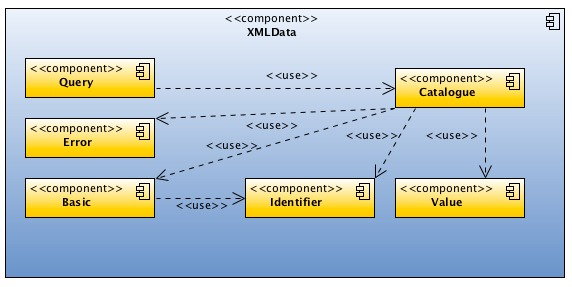
\includegraphics[width=0.82\textwidth]{images/bausteinsicht_plib_level2_xmldata.jpg}
	\caption{Bausteinsicht - Level 2 - Komponente XMLData}
	\label{fig:bausteinsicht_level2_xmldata}
\end{figure}

\begin{description}
\item[Query] Diese Komponente beinhaltet das Datenmodell des Queries nach ISO/TS 29002-31. 
\item[Catalogue] Diese Komponente beinhaltet das Datenmodell des Kataloges nach ISO/TS 29002-10. 
\item[Basic] Diese Komponente beinhaltet das Datenmodell von Basistypen nach ISO/TS 29002-4.
\item[Value] Diese Komponente beinhaltet das Datenmodell der Wertetypen nach ISO/TS 29002-10.
\item[Identifier] Diese Komponente beinhaltet das Datenmodell für Identifier (IRDI) nach ISO/TS 29002-5. 
\end{description}

\section{Level 2 - Whiteboxansicht - Komponente Processor}\index{Whiteboxansicht}

Die Komponente Processor beinhaltet den QueryProcessor sowie die Handler und Analyser-Komponente. Siehe dazu \autoref{fig:bausteinsicht_level2_processor}. 

\begin{figure}[htbp]
	\centering
		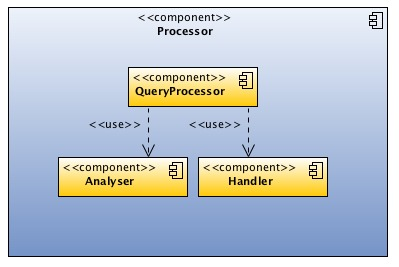
\includegraphics[width=0.70\textwidth]{images/bausteinsicht_plib_level2_processor.jpg}
	\caption{Bausteinsicht - Level 2 - Komponente Processor}
	\label{fig:bausteinsicht_level2_processor}
\end{figure}

\begin{description}
\item[QueryProcessor] Diese Komponente ist für die erste Queryverarbeitung verantwortlich. Übernimmt eine Erkennung des Queries und leitet an den Handler und Analyser weiter. 
\item[Handler] Diese Komponente beinhaltet die QueryServices, welche die eigentliche Verarbeitung und Transformation der Queries in die Datenmodelle übernimmt.
\item[Analyser] Enthält Komponenten zur Analyse und Markierung des Queries für die weitere Verarbeitung. 
\end{description}

\section{Level 3 - Whiteboxansicht - Komponente Handler}\index{Whiteboxansicht}

Die Komponente Handler beinhaltet die QueryServices, die zur Verarbeitung sowie Transformation der Queries zuständig sind. Siehe dazu \autoref{fig:bausteinsicht_level3_handler}. 

\begin{figure}[htbp]
	\centering
		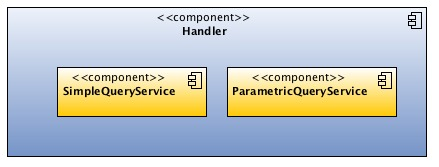
\includegraphics[width=0.82\textwidth]{images/bausteinsicht_plib_level3_handler.jpg}
	\caption{Bausteinsicht - Level 3 - Komponente Handler}
	\label{fig:bausteinsicht_level3_handler}
\end{figure}

\begin{description}
\item[SimpleQueryService] Diese Komponente ist für die Verarbeitung und Transformation der SimpleQueries (Projektion) zuständig. Bereitet die Anfrage für die Datenbank für die PLIBDao-Komponente vor. 
\item[ParametricQueryService] Diese Komponente ist für die Verarbeitung und Transformation der ParametricQueries (Selektion) zuständig. Bereitet die Anfrage für die Datenbank für die PLIBDao-Komponente vor. 
\end{description}

\section{Level 3 - Whiteboxansicht - Komponente Analyser}\index{Whiteboxansicht}

Die Komponente Analyser beinhaltet Komponenten zur Analyse und Markieren der Eingangsqueries. Siehe dazu \autoref{fig:bausteinsicht_level3_analyser}. 

\begin{figure}[htbp]
	\centering
		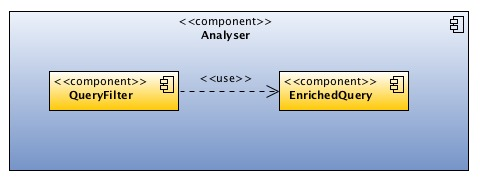
\includegraphics[width=0.82\textwidth]{images/bausteinsicht_plib_level3_analyser.jpg}
	\caption{Bausteinsicht - Level 3 - Komponente Analyser}
	\label{fig:bausteinsicht_level3_analyser}
\end{figure}

\begin{description}
\item[QueryFilter] Diese Komponente filtert den Eingangsquery und markiert ihn mit Hilfe von EnrichedQuery.
\item[EnrichedQuery] Diese Komponente markiert den Query gemäß seiner Art (Simple, Parametric) zur späteren schnellen Erkennung. Es muss somit keine aufwändige Erkennung durch Prüfen der Eingangsdaten durchgeführt werden, sondern es können Flags in dieser Komponente abgefragt werden. 
\end{description}
